\documentclass[tikz,border=5pt]{standalone}
\pdfinfoomitdate=1
\pdftrailerid{}
\pdfsuppressptexinfo=-1
\usepackage{pgfplots}
\usepgfplotslibrary{groupplots}
\pgfplotsset{compat=1.18}
\definecolor{atlasBlue}{HTML}{0072B2}
\definecolor{atlasOrange}{HTML}{E69F00}
\definecolor{atlasGreen}{HTML}{009E73}
\definecolor{atlasPurple}{HTML}{CC79A7}
\definecolor{atlasGray}{HTML}{777777}
% NATO SERS figure F46; data_sha256=455c37e7642c982d1f804c33883f563baa41751f89a87c60d0fda9821cb7ef08
% title=Same-master substrate by instrument crossover effects
% caption=Same-master difference-in-differences, oriented as the substrate-B effect at instrument B minus at instrument A. Circles are C-SELECTED and squares fixed RBF SVM; horizontal bars are 95\% master-bootstrap intervals. The distance panel is PP-U-MIN cosine-distance difference (substrate B minus A). Singleton blocks have point estimates only; unavailable predictive blocks remain visible in the semantic table.
\begin{document}
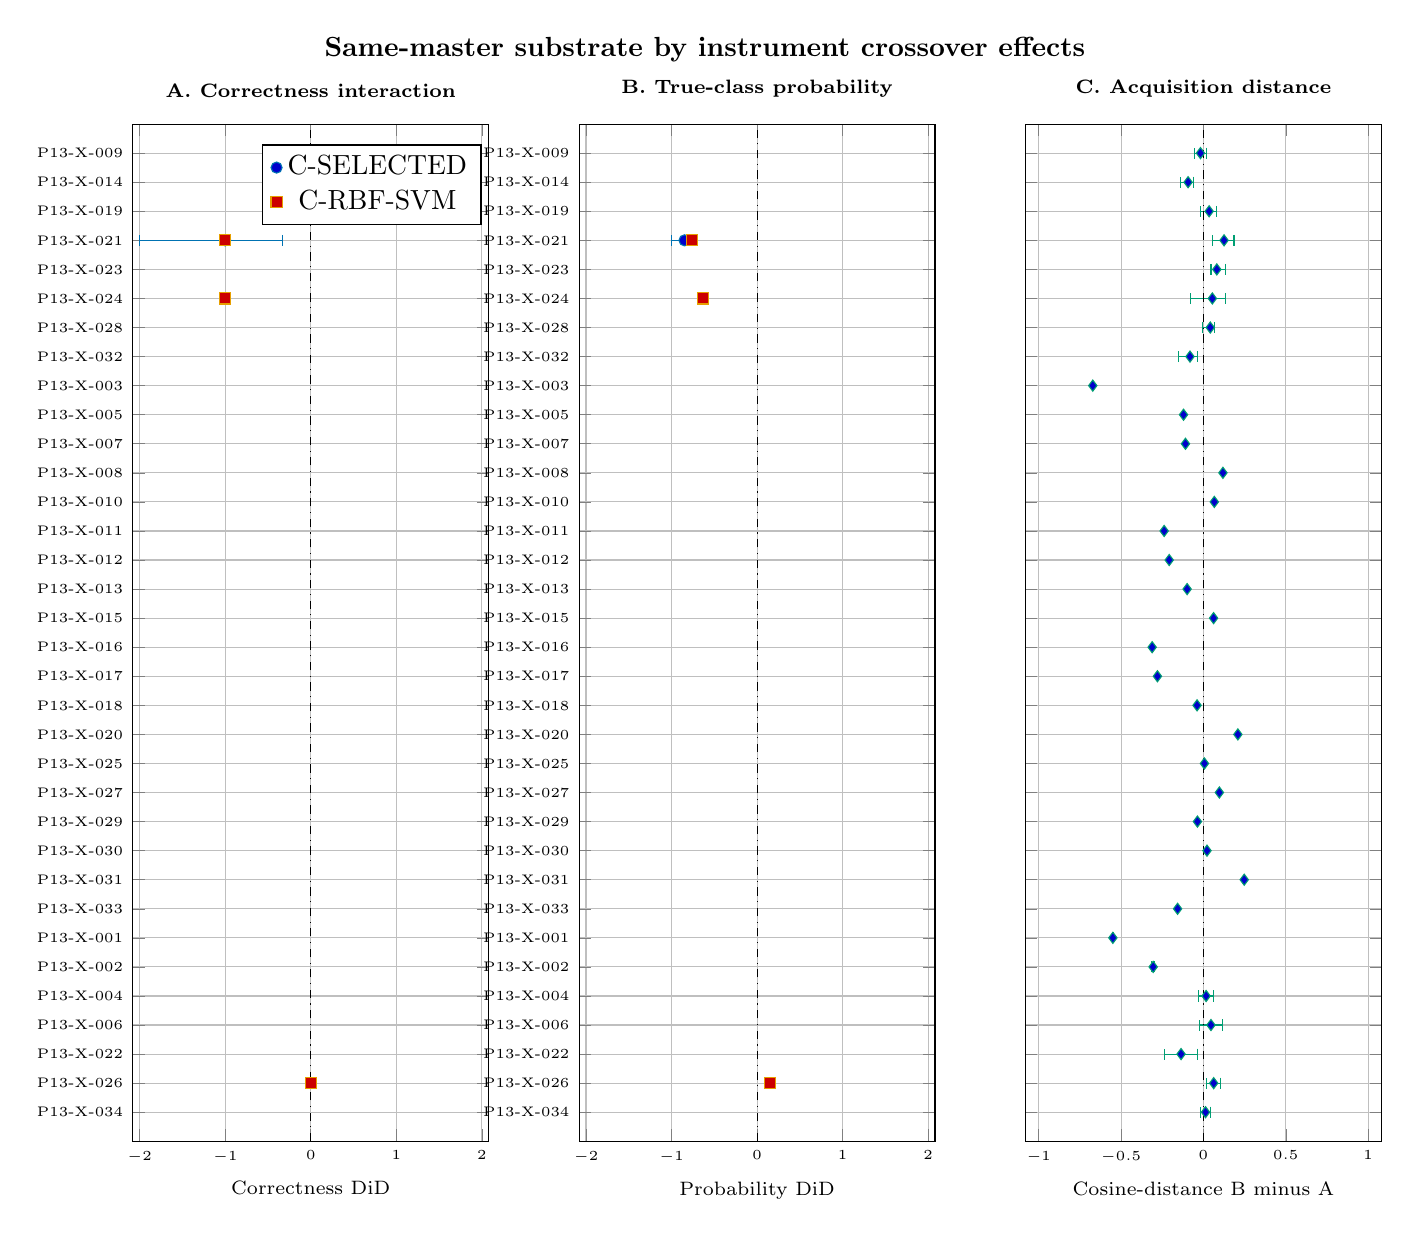
\begin{tikzpicture}
\begin{groupplot}[group style={group size=3 by 1,horizontal sep=1.15cm},width=6.1cm,height=14.5cm,
tick label style={font=\tiny},label style={font=\scriptsize},title style={font=\scriptsize\bfseries},
ytick={33,32,31,30,29,28,27,26,25,24,23,22,21,20,19,18,17,16,15,14,13,12,11,10,9,8,7,6,5,4,3,2,1,0},yticklabels={P13-X-009,P13-X-014,P13-X-019,P13-X-021,P13-X-023,P13-X-024,P13-X-028,P13-X-032,P13-X-003,P13-X-005,P13-X-007,P13-X-008,P13-X-010,P13-X-011,P13-X-012,P13-X-013,P13-X-015,P13-X-016,P13-X-017,P13-X-018,P13-X-020,P13-X-025,P13-X-027,P13-X-029,P13-X-030,P13-X-031,P13-X-033,P13-X-001,P13-X-002,P13-X-004,P13-X-006,P13-X-022,P13-X-026,P13-X-034},y tick label style={font=\tiny},grid=major]
\nextgroupplot[title={A. Correctness interaction},xlabel={Correctness DiD},xmin=-2.08,xmax=2.08,ymin=-1,ymax=34,yticklabels={P13-X-009,P13-X-014,P13-X-019,P13-X-021,P13-X-023,P13-X-024,P13-X-028,P13-X-032,P13-X-003,P13-X-005,P13-X-007,P13-X-008,P13-X-010,P13-X-011,P13-X-012,P13-X-013,P13-X-015,P13-X-016,P13-X-017,P13-X-018,P13-X-020,P13-X-025,P13-X-027,P13-X-029,P13-X-030,P13-X-031,P13-X-033,P13-X-001,P13-X-002,P13-X-004,P13-X-006,P13-X-022,P13-X-026,P13-X-034},]
\addplot+[only marks,mark=*,color=atlasBlue,error bars/.cd,x dir=both,x explicit] coordinates {(-1,30) += (0.66666667,0) -= (1,0)};
\addlegendentry{C-SELECTED}
\addplot+[only marks,mark=square*,color=atlasOrange,error bars/.cd,x dir=both,x explicit] coordinates {(-1,30) += (0,0) -= (0,0) (-1,28) += (0,0) -= (0,0) (0,1) += (0,0) -= (0,0)};
\addlegendentry{C-RBF-SVM}
\addplot[black,dashdotted] coordinates {(0,-1) (0,34)};
\nextgroupplot[title={B. True-class probability},xlabel={Probability DiD},xmin=-2.08,xmax=2.08,ymin=-1,ymax=34,]
\addplot+[only marks,mark=*,color=atlasBlue,error bars/.cd,x dir=both,x explicit] coordinates {(-0.84841487,30) += (0.081263278,0) -= (0.14971702,0)};
\addplot+[only marks,mark=square*,color=atlasOrange,error bars/.cd,x dir=both,x explicit] coordinates {(-0.76110048,30) += (0.02218338,0) -= (0.023019362,0) (-0.62810146,28) += (0.043304419,0) -= (0.058886374,0) (0.15561959,1) += (0.0066157873,0) -= (0.0066157873,0)};
\addplot[black,dashdotted] coordinates {(0,-1) (0,34)};
\nextgroupplot[title={C. Acquisition distance},xlabel={Cosine-distance B minus A},xmin=-1.08,xmax=1.08,ymin=-1,ymax=34,yticklabels={}]
\addplot+[only marks,mark=diamond*,color=atlasGreen,error bars/.cd,x dir=both,x explicit] coordinates {(-0.01793251,33) += (0.034882893,0) -= (0.037671207,0) (-0.093118908,32) += (0.031443339,0) -= (0.04685594,0) (0.034858195,31) += (0.045320919,0) -= (0.053418051,0) (0.12529394,30) += (0.060335058,0) -= (0.068782316,0) (0.081263517,29) += (0.052657465,0) -= (0.035395211,0) (0.054110238,28) += (0.08161204,0) -= (0.1312837,0) (0.041671482,27) += (0.027778585,0) -= (0.047710202,0) (-0.081470106,26) += (0.046006555,0) -= (0.072537758,0) (-0.67176194,25) (-0.1208984,24) (-0.10903731,23) (0.11848921,22) (0.066062333,21) (-0.23824783,20) (-0.20768884,19) (-0.099072466,18) (0.061733294,17) (-0.31133987,16) (-0.27919556,15) (-0.038497862,14) (0.20909476,13) (0.0061704842,12) (0.096826212,11) (-0.036376164,10) (0.021669165,9) (0.24766699,8) (-0.15669436,7) (-0.54967372,6) += (0.001654142,0) -= (0.001654142,0) (-0.30511393,5) += (0.0082999629,0) -= (0.0082999629,0) (0.016375829,4) += (0.047416562,0) -= (0.047416562,0) (0.04592707,3) += (0.07050199,0) -= (0.07050199,0) (-0.13578119,2) += (0.098285242,0) -= (0.098285242,0) (0.062392333,1) += (0.041382335,0) -= (0.041382335,0) (0.012703225,0) += (0.030676519,0) -= (0.030676519,0)};
\addplot[black,dashdotted] coordinates {(0,-1) (0,34)};
\end{groupplot}
\node[font=\normalsize\bfseries,anchor=south] at (current bounding box.north) {Same-master substrate by instrument crossover effects};
\end{tikzpicture}
\end{document}
